\begin{figure}[H]
	\centering
	\subfloat[][DCAP\_2\_2\_2\_2\_block\_A.pdf]
	{
		\centering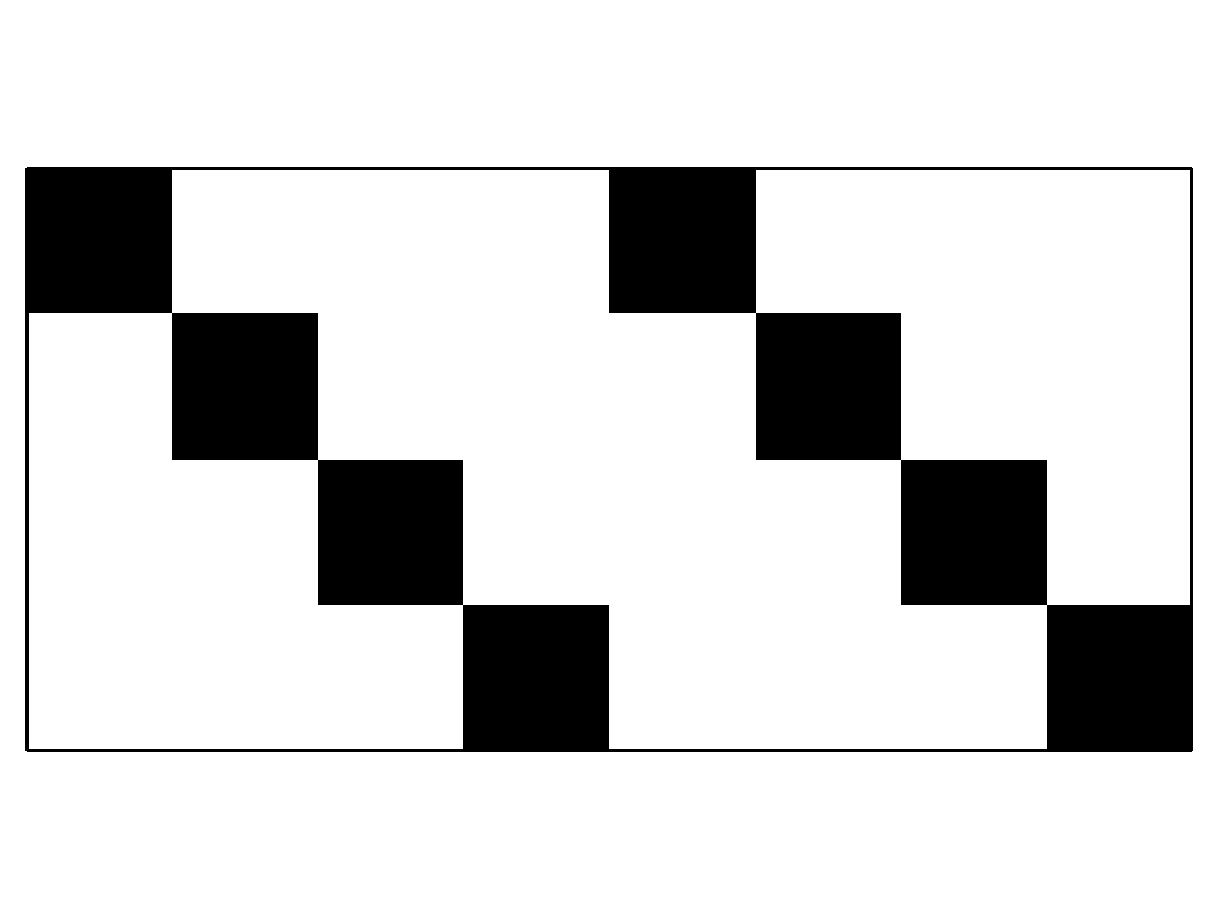
\includegraphics[width=0.45\linewidth]{DCAP_2_2_2_2_block_A}
		\label{fig:plotall_a}
	}
	~
	\subfloat[][DCAP\_2\_2\_2\_2.pdf]
	{
		\centering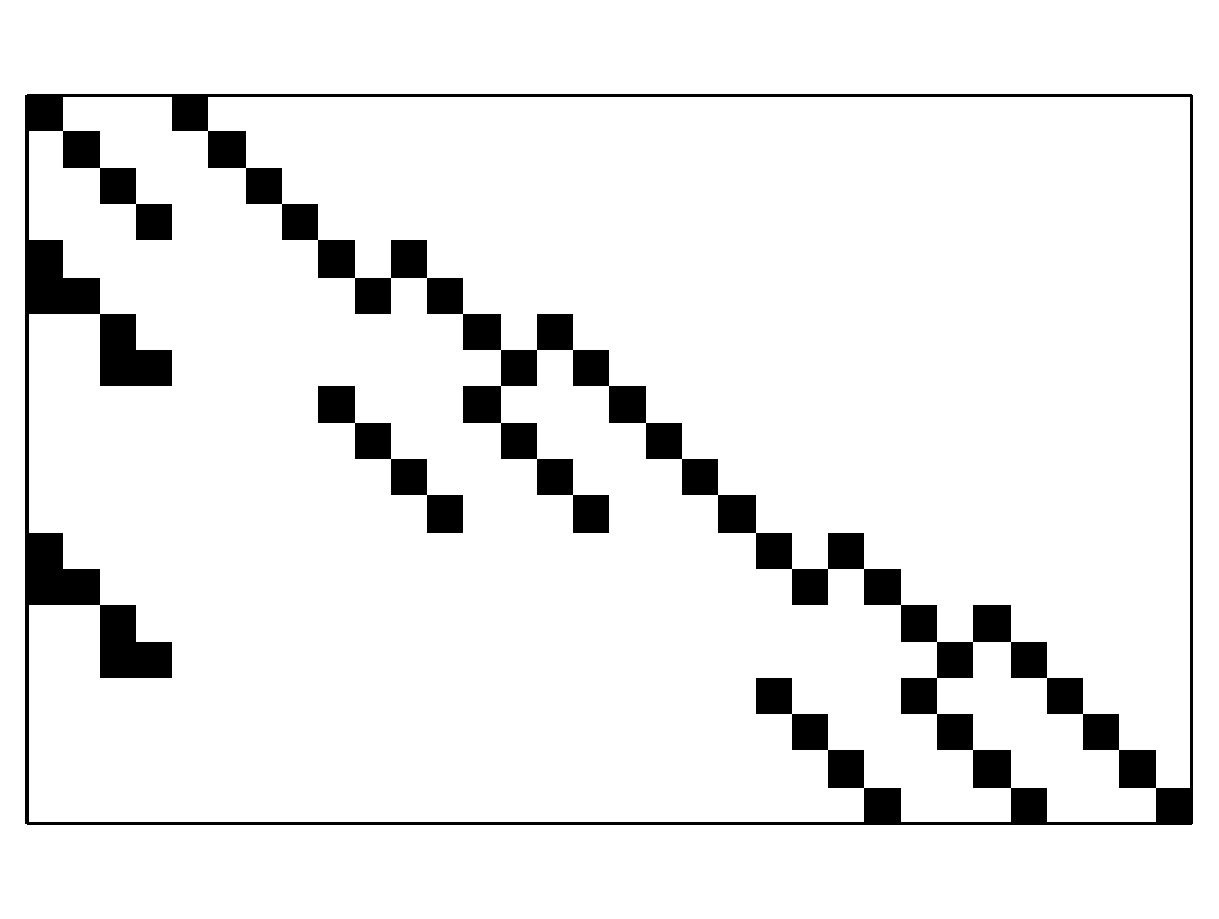
\includegraphics[width=0.45\linewidth]{DCAP_2_2_2_2}
		\label{fig:plotall_b}
	}
	
	\subfloat[][DCAP\_2\_2\_2\_2\_block\_T.pdf]
	{
		\centering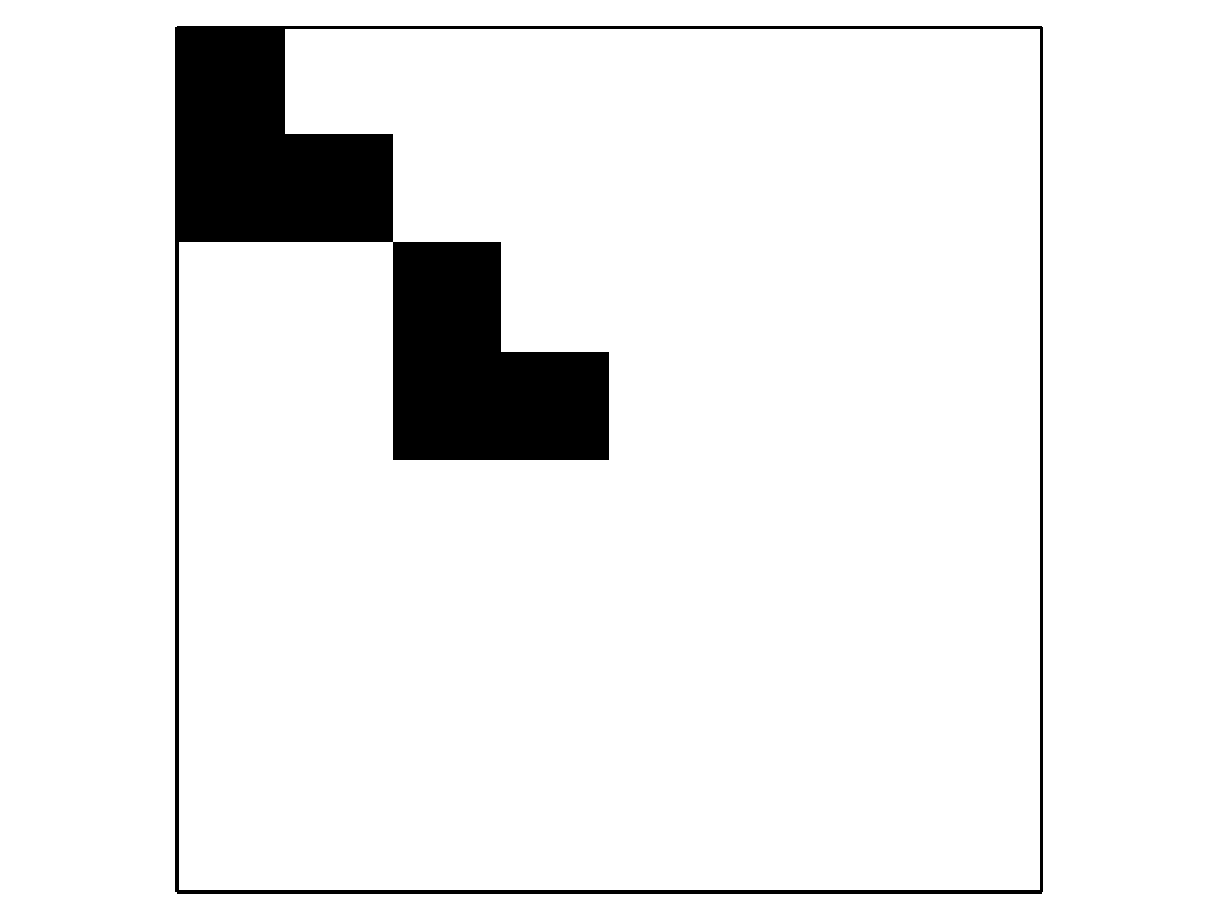
\includegraphics[width=0.45\linewidth]{DCAP_2_2_2_2_block_T}
		\label{fig:plotall_c}
	}
	~
	\subfloat[][DCAP\_2\_2\_2\_2\_block\_W.pdf]
	{
		\centering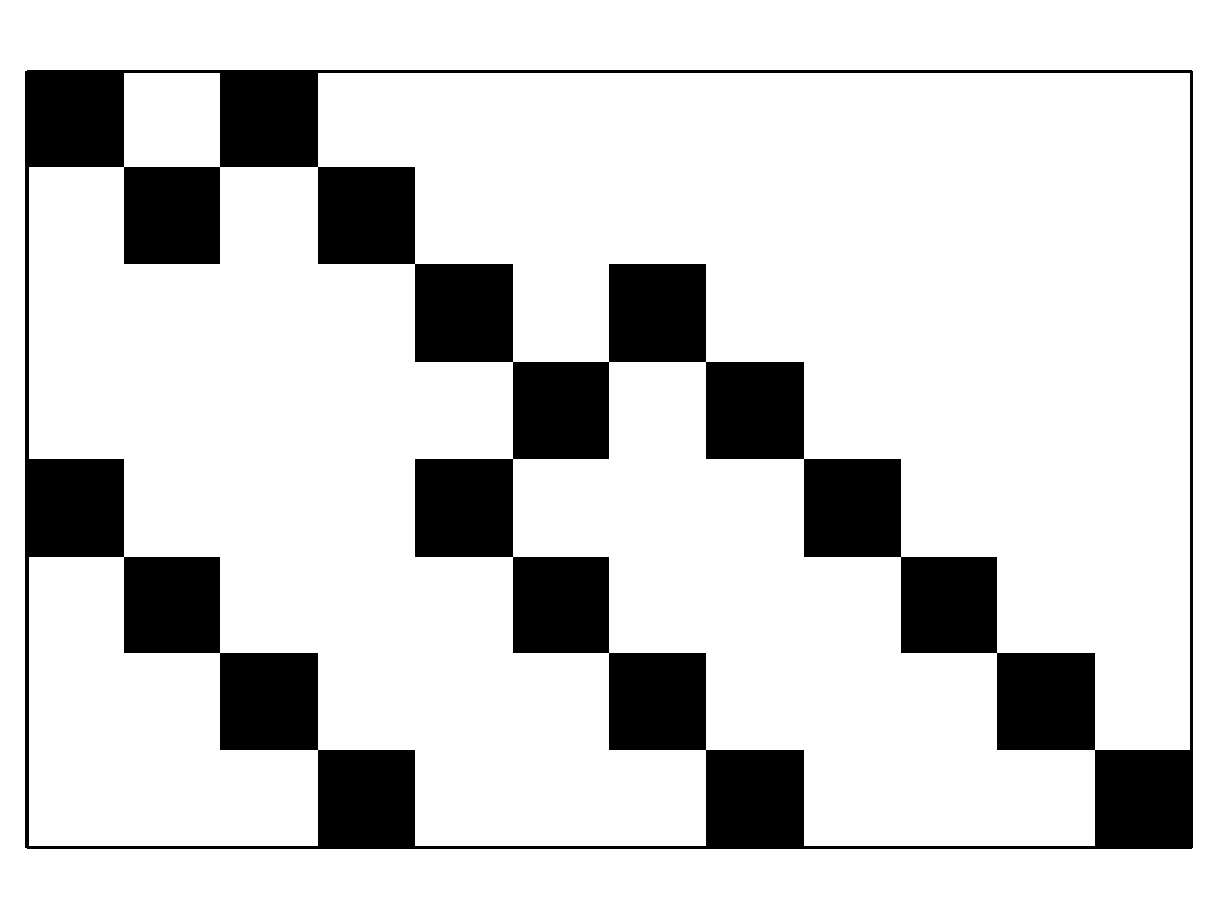
\includegraphics[width=0.45\linewidth]{DCAP_2_2_2_2_block_W}
		\label{fig:plotall_d}
	}

	\caption{Plots drawn by executing function \texttt{plotAll}}
%	\begin{minipage}
%	\end{minipage}
	\label{fig:plotall}
\end{figure}